\section{Architecture}

\begin{figure}[ht!]
  \centering
    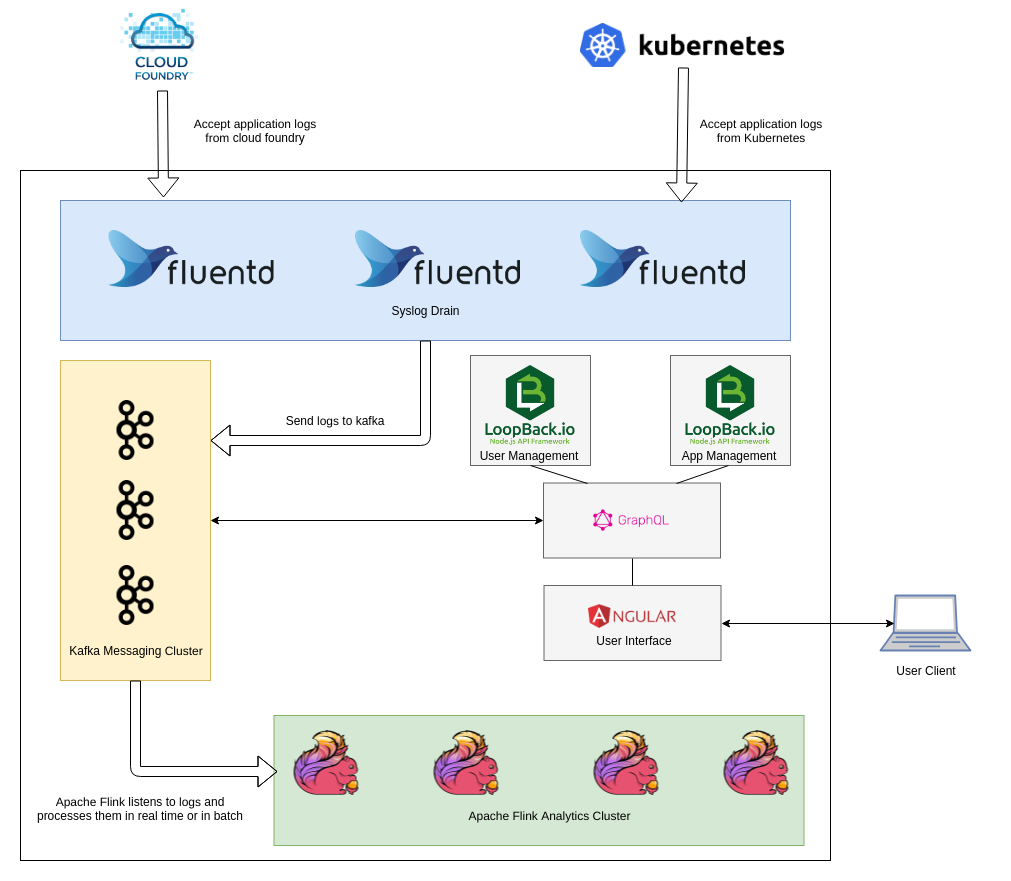
\includegraphics[width=0.5\textwidth]{images/architecture.png}
  \caption{Log analysis architecture.}
\end{figure}

\subsection{Syslog Protocol}

Log Drain is a feature of Pivotal Cloud Foundry which can be utilized to forward all logs from a particular application or multitude of applications to a central service. A Cloud Foundry operator needs to provide a URL to the service they wish to forward logs to. Log Drain uses a protocol known as syslog. This
can be used for a number of purposes, including optimizing
system performance, system auditing, and investigating malicious
activities in a computer network\cite{6827714} and supports both TCP and UDP connections.

\subsection{Fluentd}

Fluentd is a scalable open source data collector. It supports many different protocols natively, including syslog. The ultimate goal in this architecture is to accept syslog messages from a Cloud Foundry PaaS system and forward them onto a kafka cluster.

\subsection{Kafka}

Kafka is a distributed streaming platform. It was originally developed at LinkedIn to address issues with processing huge amounts of data  At at very low latency. At its core Kafka is considered a distributed commit log with the ability for other services to subscribe to changes in a particular log known as a topic. Each topic has a configurable log retention period after which time logs will be deleted from the system. This project will be utilizing Kafka for storing incoming logs from Cloud Foundry for a particular period of time until such time that they are sufficiently analyzed. 

\subsection{Flink}

Apache FLink is a real time distributed stream processing framework. It is similar to Apache Spark in that, it can work in both batch processing and streaming mode, however unlike Spark, Flink does not have a requirement of Apache Hadoop.